%iffalse
\let\negmedspace\undefined
\let\negthickspace\undefined
\documentclass[journal,12pt,onecolumn]{IEEEtran}
\usepackage{cite}
\usepackage{amsmath,amssymb,amsfonts,amsthm}
\usepackage{algorithmic}
\usepackage{graphicx}
\usepackage{textcomp}
\usepackage{xcolor}
\usepackage{txfonts}
\usepackage{listings}
\usepackage{enumitem}
\usepackage{mathtools}
\usepackage{newunicodechar}
\newunicodechar{₹}{\text{Rs.}}
\usepackage{gensymb}
\usepackage{comment}
\usepackage{mathrsfs}
\usepackage[breaklinks=true]{hyperref}
\usepackage{tkz-euclide} 
\usepackage{listings}
\usepackage{gvv}
\def\inputGnumericTable{}                                 
\usepackage[utf8]{inputenc}                              
\usepackage{color}                                         
\usepackage{array}                                        
\usepackage{longtable}                                     
\usepackage{calc}                                          
\usepackage{multirow}                                      
\usepackage{hhline}                                        
\usepackage{ifthen}                                        
\usepackage{lscape}
\newtheorem{theorem}{Theorem}[section]
\newtheorem{problem}{Problem}
\newtheorem{proposition}{Proposition}[section]
\newtheorem{lemma}{Lemma}[section]
\newtheorem{corollary}[theorem]{Corollary}
\newtheorem{example}{Example}[section]
\newtheorem{definition}[problem]{Definition}
\newcommand{\BEQA}{\begin{eqnarray}}
\newcommand{\EEQA}{\end{eqnarray}}
\newcommand{\define}{\stackrel{\triangle}{=}}
\theoremstyle{remark}
\newtheorem{rem}{Remark}
\graphicspath{ {./Figures/} }
\usepackage{float} % For the [H] float option
\usepackage{textcomp}
\usepackage{multicol}

\begin{document}
\begin{enumerate}[start=1, label=Q.\arabic*]

\item The village was nestled in a green spot, \underline{\hspace{2cm}} the ocean and the hills.

\begin{enumerate}
\begin{multicols}{4}
\item through
\item in
\item at
\item between
\end{multicols}
\end{enumerate}

\hfill{\brak{\text{GATE MA 2023}}}


\item Disagree : Protest $::$ Agree : \underline{\hspace{2cm}} \quad \brak{\text{By word meaning}}

\begin{enumerate}
\begin{multicols}{4}
\item Refuse
\item Pretext
\item Recommend
\item Refute
\end{multicols}
\end{enumerate}

\hfill{\brak{\text{GATE MA 2023}}}

\item A \brak{\text{frabjous}} number is defined as a $3$ digit number with all digits odd, and no two adjacent digits being the same. For example, $137$ is a frabjous number, while $133$ is not. How many such frabjous numbers exist?
\begin{enumerate}
\item 125
\item 720
\item 60
\item 80
\end{enumerate}

\hfill{\brak{\text{GATE MA 2023}}}


\item Which one among the following statements must be TRUE about the mean and the median of the scores of all candidates appearing for GATE $2023$?
\begin{enumerate}
\item The median is at least as large as the mean.
\item The mean is at least as large as the median.
\item At most half the candidates have a score that is larger than the median.
\item At most half the candidates have a score that is larger than the mean.
\end{enumerate}

\hfill{\brak{\text{GATE MA 2023}}}

\item In the given diagram, ovals are marked at different heights $\brak{h}$ of a hill. Which one of the following options P, Q, R, and S depicts the top view of the hill?

\begin{figure}[H]
\centering
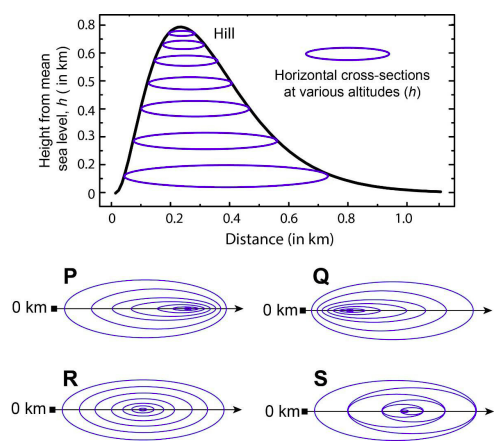
\includegraphics[width=0.7\columnwidth]{Figures/qu5.png}
\caption{}
\end{figure}

\begin{enumerate}
\begin{multicols}{4}
\item P
\item Q
\item R
\item S
\end{multicols}
\end{enumerate}

\hfill{\brak{\text{GATE MA 2023}}}
\item Residency is a famous housing complex with many well\mbox{-}established individuals among its residents. A recent survey conducted among the residents of the complex revealed that all of those residents who are well established in their respective fields happen to be academicians. The survey also revealed that most of these academicians are authors of some best\mbox{-}selling books. Based only on the information provided above, which one of the following statements can be logically inferred with certainty?
\begin{enumerate}
\item Some residents of the complex who are well established in their fields are also authors of some best\mbox{-}selling books.
\item All academicians residing in the complex are well established in their fields.
\item Some authors of best\mbox{-}selling books are residents of the complex who are well established in their fields.
\item Some academicians residing in the complex are well established in their fields.
\end{enumerate}

\hfill{\brak{\text{GATE MA 2023}}}

\item Ankita has to climb $5$ stairs starting at the ground, while respecting the following rules:
\begin{enumerate}
\item At any stage, Ankita can move either one or two stairs up.
\item At any stage, Ankita cannot move to a lower step.
\end{enumerate}

Let $F(N)$ denote the number of possible ways in which Ankita can reach the $N^{th}$ stair. For example, $F(1) = 1, \; F(2) = 2, \; F(3) = 3$. The value of $F(5)$ is \underline{\hspace{2cm}}.

\begin{enumerate}
\begin{multicols}{4}
\item 8
\item 7
\item 6
\item 5
\end{multicols}
\end{enumerate}

\hfill{\brak{\text{GATE MA 2023}}}
\item The information contained in DNA is used to synthesize proteins that are necessary for the functioning of life. DNA is composed of four nucleotides\brak{:} Adenine \brak{A}, Thymine \brak{T}, Cytosine \brak{C}, and Guanine \brak{G}. The information contained in DNA can then be thought of as a sequence of these four nucleotides\brak{:} A, T, C, and G. DNA has coding and non\mbox{-}coding regions. Coding regions\brak{—where the sequence of these nucleotides are read in groups of three to produce individual amino acids—}constitute only about $2\%$ of human DNA. For example, the triplet of nucleotides CCG codes for the amino acid glycine, while the triplet GGA codes for the amino acid proline. Multiple amino acids are then assembled to form a protein.

Based only on the information provided above, which of the following statements can be logically inferred with \textit{certainty}?
\[
\text{\brak{i}} \ \ \text{The majority of human DNA has no role in the synthesis of proteins.}
\]
\[
\text{\brak{ii}} \ \ \text{The function of about $98\%$ of human DNA is not understood.}
\]

\begin{enumerate}
\item only \brak{i}
\item only \brak{ii}
\item both \brak{i} and \brak{ii}
\item neither \brak{i} nor \brak{ii}
\end{enumerate}

\hfill{\brak{\text{GATE MA 2023}}}
\item Which one of the given figures P, Q, R and S represents the graph of the following function?
\[
f(x)=\abs{\abs{x+2}-\abs{x-1}}
\]

\begin{figure}[H]
\centering
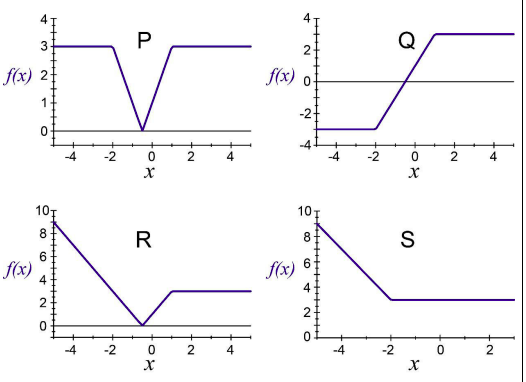
\includegraphics[width=0.9\columnwidth]{Figures/qu9.png} 
\caption{}
\end{figure}

\begin{enumerate}
\begin{multicols}{4}
\item P
\item Q
\item R
\item S
\end{multicols}
\end{enumerate}

\hfill{\brak{\text{GATE MA 2023}}}


\item An opaque cylinder is suspended in the path of a parallel beam of light, such that its shadow is cast on a screen oriented perpendicular to the direction of the light beam. The cylinder can be reoriented in any direction within the light beam. Under these conditions, which one of the shadows P, Q, R, and S is NOT possible?

\begin{figure}[H]
\centering
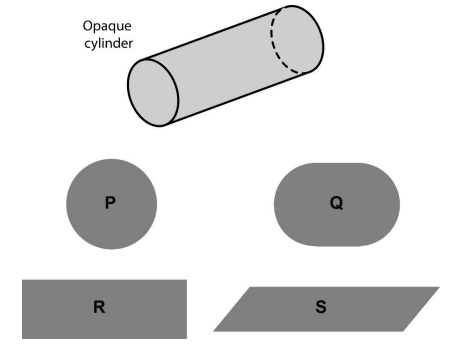
\includegraphics[width=0.9\columnwidth]{Figures/qu10.png}
\caption{}
\end{figure}

\begin{enumerate}
\begin{multicols}{4}
\item P
\item Q
\item R
\item S
\end{multicols}
\end{enumerate}

\hfill{\brak{\text{GATE MA 2023}}}
\item Let $f,\ g : \mathbb{R}^{2}\to \mathbb{R}$ be defined by
\[
f(x,y)=x^{2}-\tfrac{3}{2}\,x y^{2} \quad \text{and} \quad g(x,y)=4x^{4}-5x^{2}y+y^{2}
\]
for all $\brak{x,y}\in \mathbb{R}^{2}$. Consider the following statements\brak{:}

P : $f$ has a saddle point at $\brak{0,0}$.\\
Q : $g$ has a saddle point at $\brak{0,0}$.\\

Then
\begin{enumerate}
\item both P and Q are TRUE
\item P is FALSE but Q is TRUE
\item P is TRUE but Q is FALSE
\item both P and Q are FALSE
\end{enumerate}

\hfill{\brak{\text{GATE MA 2023}}}
\item Let $\mathbb{R}^{3}$ be a topological space with the usual topology and $\mathbb{Q}$ denote the set of rational numbers. Define the subspaces $X,Y,Z$ and $W$ of $\mathbb{R}^{3}$ as follows\brak{:}
\[
X=\{(x,y,z)\in \mathbb{R}^{3} : \abs{x}+\abs{y}+\abs{z}\in \mathbb{Q}\},
\]
\[
Y=\{(x,y,z)\in \mathbb{R}^{3} : xyz=1\},
\]
\[
Z=\{(x,y,z)\in \mathbb{R}^{3} : x^{2}+y^{2}+z^{2}=1\},
\]
\[
W=\{(x,y,z)\in \mathbb{R}^{3} : xyz=0\}.
\]
Which of the following statements is correct?
\begin{enumerate}
\begin{multicols}{2}
\item $X$ is homeomorphic to $Y$
\item $Z$ is homeomorphic to $W$
\item $Y$ is homeomorphic to $W$
\item $X$ is NOT homeomorphic to $W$
\end{multicols}
\end{enumerate}

\hfill{\brak{\text{GATE MA 2023}}}


\item Let $P(x)=1+e^{2\pi i x}+2e^{3\pi i x},\ x\in \mathbb{R},\ i=\sqrt{-1}$. Then
\[
\lim_{N\to\infty}\frac{1}{N}\sum_{k=0}^{N-1} P\!\brak{k\sqrt{2}}
\]
is equal to
\begin{enumerate}
\begin{multicols}{4}
\item $0$
\item $1$
\item $3$
\item $4$
\end{multicols}
\end{enumerate}

\hfill{\brak{\text{GATE MA 2023}}}
\item Let $T : \mathbb{R}^{3}\to \mathbb{R}^{3}$ be a linear transformation satisfying
\[
T\brak{1,0,0}=\brak{0,1,1},\qquad
T\brak{1,1,0}=\brak{1,0,1},\qquad
T\brak{1,1,1}=\brak{1,1,2}.
\]
Then
\begin{enumerate}
\begin{multicols}{2}
\item $T$ is one\mbox{-}one but $T$ is NOT onto
\item $T$ is one\mbox{-}one and onto
\item $T$ is NEITHER one\mbox{-}one NOR onto
\item $T$ is NOT one\mbox{-}one but $T$ is onto
\end{multicols}
\end{enumerate}

\hfill{\brak{\text{GATE MA 2023}}}


\item Let $\mathbb{D}=\{\, z \in \mathbb{C} : \abs{z}<1 \,\}$ and $f : \mathbb{D}\to \mathbb{C}$ be defined by
\[
f(z)= z - 25 z^{3} + \frac{z^{5}}{5!} + \frac{z^{7}}{7!} + \frac{z^{9}}{9!} - \frac{z^{11}}{11!}.
\]
Consider the following statements\brak{:}

P : $f$ has three zeros \brak{\text{counting multiplicity}} in $\mathbb{D}$.\\
Q : $f$ has one zero in $U=\{\, z \in \mathbb{C} : \tfrac{1}{2}<\abs{z}<1 \,\}$.\\

Then
\begin{enumerate}
\begin{multicols}{2}
\item P is TRUE but Q is FALSE
\item P is FALSE but Q is TRUE
\item both P and Q are TRUE
\item both P and Q are FALSE
\end{multicols}
\end{enumerate}

\hfill{\brak{\text{GATE MA 2023}}}

\item Let $\mathcal{N} \subseteq \mathbb{R}$ be a non\mbox{-}measurable set with respect to the Lebesgue measure on $\mathbb{R}$. Consider the following statements\brak{:}

P : If $M=\{x \in \mathcal{N} : x \text{ is irrational}\}$, then $M$ is Lebesgue measurable.\\
Q : The boundary of $\mathcal{N}$ has positive Lebesgue outer measure.\\

Then
\begin{enumerate}
\item both P and Q are TRUE
\item P is FALSE and Q is TRUE
\item P is TRUE and Q is FALSE
\item both P and Q are FALSE
\end{enumerate}

\hfill{\brak{\text{GATE MA 2023}}}


\item For $k \in \mathbb{N}$, let $E_{k}$ be a measurable subset of $\brak{0,1}$ with Lebesgue measure $\dfrac{1}{k^{2}}$. Define
\[
E=\bigcap_{n=1}^{\infty} \ \bigcup_{k=n}^{\infty} E_{k}
\qquad \text{and} \qquad
F=\bigcup_{n=1}^{\infty} \ \bigcap_{k=n}^{\infty} E_{k}.
\]
Consider the following statements\brak{:}

P : Lebesgue measure of $E$ is equal to zero.\\
Q : Lebesgue measure of $F$ is equal to zero.\\

Then
\begin{enumerate}
\item both P and Q are TRUE
\item both P and Q are FALSE
\item P is TRUE but Q is FALSE
\item Q is TRUE but P is FALSE
\end{enumerate}

\hfill{\brak{\text{GATE MA 2023}}}

\item Consider $\mathbb{R}^{2}$ with the usual Euclidean metric. Let
\[
X=\left\{(x, x\sin \tfrac{1}{x}) \in \mathbb{R}^{2} : x \in \brak{0,1]}\right\}\ \cup\ \left\{(0,y) \in \mathbb{R}^{2} : -\infty<y<\infty\right\}
\]
and
\[
Y=\left\{(x, \sin \tfrac{1}{x}) \in \mathbb{R}^{2} : x \in \brak{0,1]}\right\}\ \cup\ \left\{(0,y) \in \mathbb{R}^{2} : -\infty<y<\infty\right\}.
\]
Consider the following statements\brak{:}

P : $X$ is a connected subset of $\mathbb{R}^{2}$.\\
Q : $Y$ is a connected subset of $\mathbb{R}^{2}$.\\

Then
\begin{enumerate}
\item both P and Q are TRUE
\item P is FALSE and Q is TRUE
\item P is TRUE and Q is FALSE
\item both P and Q are FALSE
\end{enumerate}

\hfill{\brak{\text{GATE MA 2023}}}


\item Let $M=\myvec{4 & -3\\ 1 & 0}$. Consider the following statements\brak{:}

P : $M^{8}+M^{12}$ is diagonalizable.\\
Q : $M^{7}+M^{9}$ is diagonalizable.\\

Which of the following statements is correct?
\begin{enumerate}
\item P is TRUE and Q is FALSE
\item P is FALSE and Q is TRUE
\item Both P and Q are FALSE
\item Both P and Q are TRUE
\end{enumerate}

\hfill{\brak{\text{GATE MA 2023}}}


\item Let $C[0,1]=\{\, f : [0,1]\to \mathbb{R} \mid f \text{ is continuous}\,\}$.  
Consider the metric space $\brak{C[0,1], d_{\infty}}$, where
\[
d_{\infty}(f,g)=\sup\{\abs{f(x)-g(x)} : x \in [0,1]\}, \ \text{for } f,g \in C[0,1].
\]
Let $f_{0}(x)=0$ for all $x \in [0,1]$ and
\[
X=\Big\{\, f \in \brak{C[0,1], d_{\infty}} : d_{\infty}\!\brak{f_{0},f}\ge \tfrac{1}{2}\,\Big\}.
\]
Let $f_{1}, f_{2} \in C[0,1]$ be defined by $f_{1}(x)=x$ and $f_{2}(x)=1-x$ for all $x \in [0,1]$.  

Consider the following statements\brak{:}

P : $f_{1}$ is in the interior of $X$.\\
Q : $f_{2}$ is in the interior of $X$.\\

Which of the following statements is correct?
\begin{enumerate}
\item P is TRUE and Q is FALSE
\item P is FALSE and Q is TRUE
\item Both P and Q are FALSE
\item Both P and Q are TRUE
\end{enumerate}

\hfill{\brak{\text{GATE MA 2023}}}


\item Consider the metrics $\rho_{1}$ and $\rho_{2}$ on $\mathbb{R}$, defined by
\[
\rho_{1}(x,y)=\abs{x-y}
\quad \text{and} \quad
\rho_{2}(x,y)=
\begin{cases}
0, & x=y,\\
1, & x\ne y.
\end{cases}
\]
Let $X=\{\, n \in \mathbb{N} : n \ge 3 \,\}$ and $Y=\{\, 2+\tfrac{1}{n} : n \in \mathbb{N} \,\}$.  
Define $f : X \cup Y \to \mathbb{R}$ by
\[
f(x)=
\begin{cases}
2, & \text{if } x \in X,\\
3, & \text{if } x \in Y.
\end{cases}
\]

Consider the following statements\brak{:}

P : The function $f : \brak{X \cup Y,\rho_{1}} \to \brak{\mathbb{R},\rho_{1}}$ is uniformly continuous.\\
Q : The function $f : \brak{X \cup Y,\rho_{2}} \to \brak{\mathbb{R},\rho_{1}}$ is uniformly continuous.\\

Then
\begin{enumerate}
\item P is TRUE and Q is FALSE
\item P is FALSE and Q is TRUE
\item both P and Q are FALSE
\item both P and Q are TRUE
\end{enumerate}

\hfill{\brak{\text{GATE MA 2023}}}

\item Let $T : \mathbb{R}^{4}\to \mathbb{R}^{4}$ be a linear transformation and the null space of $T$ be the subspace of $\mathbb{R}^{4}$ given by
\[
\{\, (x_{1},x_{2},x_{3},x_{4})\in \mathbb{R}^{4} : 4x_{1}+3x_{2}+2x_{3}+x_{4}=0 \,\}.
\]
If $\operatorname{Rank}\!\brak{T-3I}=3$, where $I$ is the identity map on $\mathbb{R}^{4}$, then the minimal polynomial of $T$ is
\begin{enumerate}
\begin{multicols}{2}
\item $x\brak{x-3}$
\item $x\brak{x-3}^{3}$
\item $x^{3}\brak{x-3}$
\item $x^{2}\brak{x-3}^{2}$
\end{multicols}
\end{enumerate}

\hfill{\brak{\text{GATE MA 2023}}}


\item Let $C[0,1]$ denote the set of all real valued continuous functions defined on $\brak{0,1}$ and $\lVert f\rVert_{\infty}=\sup\{\abs{f(x)} : x\in [0,1]\}$ for all $f\in C[0,1]$.  
Let
\[
X=\{\, f\in C[0,1] : f(0)=f(1)=0 \,\}.
\]
Define $F : \brak{C[0,1],\lVert \cdot \rVert_{\infty}}\to \mathbb{R}$ by $F(f)=\int_{0}^{1} f(t)\,dt$ for all $f\in C[0,1]$.  
Denote $S_{X}=\{\, f\in X : \lVert f\rVert_{\infty}=1 \,\}$.  

Then the set $\{\, f\in X : F(f)=\lVert F\rVert \,\}\cap S_{X}$ has
\begin{enumerate}
\item NO element
\item exactly one element
\item exactly two elements
\item an infinite number of elements
\end{enumerate}

\hfill{\brak{\text{GATE MA 2023}}}

\item Let $X$ and $Y$ be two topological spaces. A continuous map $f : X\to Y$ is said to be proper if $f^{-1}(K)$ is compact in $X$ for every compact subset $K$ of $Y$, where $f^{-1}(K)$ is defined by $f^{-1}(K)=\{\, x\in X : f(x)\in K \,\}$.  

Consider $\mathbb{R}$ with the usual topology. If $\mathbb{R}\setminus \{0\}$ has the subspace topology induced from $\mathbb{R}$ and $\mathbb{R}\times \mathbb{R}$ has the product topology, then which of the following maps is proper?
\begin{enumerate}
\item $f : \mathbb{R}\setminus \{0\}\to \mathbb{R}$ defined by $f(x)=x$
\item $f : \mathbb{R}\times \mathbb{R}\to \mathbb{R}\times \mathbb{R}$ defined by $f(x,y)=(x+y,y)$
\item $f : \mathbb{R}\times \mathbb{R}\to \mathbb{R}$ defined by $f(x,y)=x$
\item $f : \mathbb{R}\times \mathbb{R}\to \mathbb{R}$ defined by $f(x,y)=x^{2}-y^{2}$
\end{enumerate}

\hfill{\brak{\text{GATE MA 2023}}}

\item Consider the following Linear Programming Problem $P$:  
\[
\text{Minimize } 3x_{1}+4x_{2}
\]
subject to
\[
x_{1}-x_{2}\leq 1,\quad x_{1}+x_{2}\geq 3,\quad x_{1}\geq 0,\;x_{2}\geq 0.
\]
The optimal value of the problem $P$ is \_\_\_\_\_\_\_\_\_.

\hfill{\brak{\text{GATE MA 2023}}}

\item Let $u(x,t)$ be the solution of
\[
\dfrac{\partial^{2}u}{\partial x^{2}}-\dfrac{1}{c^{2}}\dfrac{\partial^{2}u}{\partial t^{2}}=0,\quad x \in \brak{-\infty,\infty},\ t>0,
\]
\[
u(x,0)=\sin x,\quad x \in \brak{-\infty,\infty},
\]
\[
\dfrac{\partial u}{\partial t}(x,0)=\cos x,\quad x \in \brak{-\infty,\infty},
\]
for some positive real number $c$.  

Let the domain of dependence of the solution $u$ at the point $P\brak{3,2}$ be the line segment on the $x$\mbox{-}axis with end points $Q$ and $R$. If the area of the triangle $PQR$ is $8$ square units, then the value of $c^{2}$ is \underline{\hspace{2cm}}.

\hfill{\brak{\text{GATE MA 2023}}}


\item Let
\[
\dfrac{z}{1-z-z^{2}}=\sum_{n=0}^{\infty} a_{n} z^{n},\qquad a_{n}\in \mathbb{R},
\]
for all $z$ in some neighbourhood of $0$ in $\mathbb{C}$. Then the value of $a_{6}+a_{5}$ is equal to \underline{\hspace{2cm}}.

\hfill{\brak{\text{GATE MA 2023}}}
\item Let $p(x)=x^{3}-2x+2$. If $q(x)$ is the interpolating polynomial of degree less than or equal to $4$ for the data
\begin{table}[H]
\centering
\caption*{}
\label{tab:q28data}
\begin{tabular}{c|ccccc}
$x$ & $-2$ & $-1$ & $0$ & $1$ & $3$ \\
\hline
$q(x)$ & $p(-2)$ & $p(-1)$ & $2.5$ & $p(1)$ & $p(3)$
\end{tabular}
\end{table}
then the value of $\dfrac{d^{4}q}{dx^{4}}$ at $x=0$ is \underline{\hspace{2cm}}.

\hfill{\brak{\text{GATE MA 2023}}}


\item For a fixed $c \in \mathbb{R}$, let $\alpha=\displaystyle \int_{0}^{2}\!\brak{9x^{2}-5cx^{4}}\,dx$. If the value of $\displaystyle \int_{0}^{2}\!\brak{9x^{2}-5cx^{4}}\,dx$ obtained by using the Trapezoidal rule is equal to $\alpha$, then the value of $c$ is \underline{\hspace{2cm}} \brak{\text{rounded off to } 2 \text{ decimal places}}.

\hfill{\brak{\text{GATE MA 2023}}}


\item If for some $\alpha \in \mathbb{R}$,
\[
\int_{1}^{4}\int_{-x}^{x}\frac{1}{x^{2}+y^{2}}\,dy\,dx
=
\int_{-\pi/4}^{\pi/4}\int_{\sec\theta}^{\alpha \sec\theta}\frac{1}{r}\,dr\,d\theta,
\]
then the value of $\alpha$ equals \underline{\hspace{2cm}}.

\hfill{\brak{\text{GATE MA 2023}}}


\item Let $S$ be the portion of the plane $z=2x+2y-100$ which lies inside the cylinder $x^{2}+y^{2}=1$. If the surface area of $S$ is $\alpha \pi$, then the value of $\alpha$ is equal to \underline{\hspace{2cm}}.

\hfill{\brak{\text{GATE MA 2023}}}


\item Let $L^{2}\brak{-1,1}=\{\, f : [-1,1]\to \mathbb{R} : f \text{ is Lebesgue measurable and } \int_{-1}^{1}\abs{f(x)}^{2}dx<\infty \,\}$ and the norm $\lVert f\rVert_{2}=\left(\int_{-1}^{1}\abs{f(x)}^{2}dx\right)^{\tfrac{1}{2}}$ for $f\in L^{2}\brak{-1,1}$.  

Let $F: \brak{L^{2}\brak{-1,1},\lVert\cdot\rVert_{2}}\to \mathbb{R}$ be defined by
\[
F(f)=\int_{-1}^{1}f(x)\,x^{2}\,dx \quad \text{for all } f\in L^{2}\brak{-1,1}.
\]
If $\lVert F\rVert$ denotes the norm of the linear functional $F$, then $5\lVert F\rVert^{2}$ is equal to \underline{\hspace{2cm}}.

\hfill{\brak{\text{GATE MA 2023}}}


\item Let $y(t)$ be the solution of the initial value problem
\[
y''+4y=
\begin{cases}
t, & 0\le t\le 2,\\
2, & 2<t<\infty,
\end{cases}
\qquad
y(0)=y'(0)=0.
\]
If $\alpha=y\!\brak{\tfrac{\pi}{2}}$, then the value of $\dfrac{4}{\pi}\alpha$ is \underline{\hspace{2cm}} \brak{\text{rounded off to } 2 \text{ decimal places}}.

\hfill{\brak{\text{GATE MA 2023}}}


\item Consider $\mathbb{R}^{4}$ with the inner product $\langle x,y\rangle=\sum_{i=1}^{4}x_{i}y_{i}$, for $x=\brak{x_{1},x_{2},x_{3},x_{4}}$ and $y=\brak{y_{1},y_{2},y_{3},y_{4}}$.  

Let $M=\{\, \brak{x_{1},x_{2},x_{3},x_{4}}\in \mathbb{R}^{4} : x_{1}=x_{3}\,\}$ and let $M^{\perp}$ denote the orthogonal complement of $M$. The dimension of $M^{\perp}$ is equal to \underline{\hspace{2cm}}.

\hfill{\brak{\text{GATE MA 2023}}}


\item Let
\[
M=\myvec{3 & -1 & -2\\ 0 & 2 & 4\\ 0 & 0 & 1}
\quad \text{and} \quad
I=\myvec{1 & 0 & 0\\ 0 & 1 & 0\\ 0 & 0 & 1}.
\]
If $6M^{-1}=M^{2}-6M+\alpha I$ for some $\alpha \in \mathbb{R}$, then the value of $\alpha$ is equal to \underline{\hspace{2cm}}.

\hfill{\brak{\text{GATE MA 2023}}}

\item Let $GL_{2}(\mathbb{C})$ denote the group of $2 \times 2$ invertible complex matrices with usual matrix multiplication. For $S, T \in GL_{2}(\mathbb{C})$, $<S, T>$ denotes the subgroup generated by $S$ and $T$. Let 
\[
S = \begin{bmatrix} 0 & -1 \\ 1 & 0 \end{bmatrix} \in GL_{2}(\mathbb{C})
\]
and $G_{1}, G_{2}, G_{3}$ be three subgroups of $GL_{2}(\mathbb{C})$ given by 
\[
G_{1} = <S, T_{1}>, \quad \text{where } T_{1} = \begin{bmatrix} i & 0 \\ 0 & i \end{bmatrix},
\]
\[
G_{2} = <S, T_{2}>, \quad \text{where } T_{2} = \begin{bmatrix} i & 0 \\ 0 & -i \end{bmatrix},
\]
\[
G_{3} = <S, T_{3}>, \quad \text{where } T_{3} = \begin{bmatrix} 0 & 1 \\ 1 & 0 \end{bmatrix}.
\]

Let $Z(G_{i})$ denote the center of $G_{i}$ for $i = 1, 2, 3$.  
Which of the following statements is correct?

\begin{enumerate}
\item $G_{1}$ is isomorphic to $G_{3}$
\item $Z(G_{1})$ is isomorphic to $Z(G_{2})$
\item $Z(G_{3}) = \left\{ \begin{bmatrix} 1 & 0 \\ 0 & 1 \end{bmatrix} \right\}$
\item $Z(G_{2})$ is isomorphic to $Z(G_{3})$
\end{enumerate}


% Q.37
\item Let $\ell^{2} = \{(x_{1}, x_{2}, x_{3}, \dots) : x_{n} \in \mathbb{R} \ \forall n \in \mathbb{N} \text{ and } \sum_{n=1}^{\infty} x_{n}^{2} < \infty \}$.

For a sequence $(x_{1}, x_{2}, x_{3}, \dots) \in \ell^{2}$, define $\|(x_{1}, x_{2}, x_{3}, \dots)\|_{2} = \left(\sum_{n=1}^{\infty} x_{n}^{2}\right)^{1/2}$.

Let $S : (\ell^{2}, \|\cdot\|_{2}) \to (\ell^{2}, \|\cdot\|_{2})$ and $T : (\ell^{2}, \|\cdot\|_{2}) \to (\ell^{2}, \|\cdot\|_{2})$ be defined by
\[
S(x_{1}, x_{2}, x_{3}, \dots) = (y_{1}, y_{2}, y_{3}, \dots), \quad \text{where } y_{n} = \begin{cases} 
0, & n=1, \\
x_{n-1}, & n \geq 2,
\end{cases}
\]
\[
T(x_{1}, x_{2}, x_{3}, \dots) = (y_{1}, y_{2}, y_{3}, \dots), \quad \text{where } y_{n} = \begin{cases}
0, & n \text{ is odd}, \\
x_{n}, & n \text{ is even}.
\end{cases}
\]

Then

\begin{enumerate}
\item $S$ is a compact linear map and $T$ is NOT a compact linear map
\item $S$ is NOT a compact linear map and $T$ is a compact linear map
\item Both $S$ and $T$ are compact linear maps
\item Neither $S$ nor $T$ is a compact linear map
\end{enumerate}
\hfill{\brak{\text{GATE MA 2023}}}
\item Let $c_{00}=\{(x_{1},x_{2},x_{3},\dots): x_{i}\in \mathbb{R},\ i\in \mathbb{N},\ x_{i}\ne 0 \text{ only for finitely many indices } i\}$.  
For $(x_{1},x_{2},x_{3},\dots)\in c_{00}$, let $\lVert(x_{1},x_{2},x_{3},\dots)\rVert_{\infty}=\sup\{|x_{i}|: i\in \mathbb{N}\}$.  

Define $F,G:(c_{00},\lVert\cdot\rVert_{\infty})\to(c_{00},\lVert\cdot\rVert_{\infty})$ by
\[
F\big((x_{1},x_{2},\dots,x_{n},\dots)\big)=\big((1+1)x_{1},\ (2+\tfrac{1}{2})x_{2},\ \dots,\ (n+\tfrac{1}{n})x_{n},\dots\big),
\]
\[
G\big((x_{1},x_{2},\dots,x_{n},\dots)\big)=\big(\tfrac{x_{1}}{1+1},\ \tfrac{x_{2}}{2+\tfrac{1}{2}},\ \dots,\ \tfrac{x_{n}}{n+\tfrac{1}{n}},\dots\big),
\]
for all $(x_{1},x_{2},\dots,x_{n},\dots)\in c_{00}$. Then
\begin{enumerate}
\item $F$ is continuous but $G$ is NOT continuous
\item $F$ is NOT continuous but $G$ is continuous
\item both $F$ and $G$ are continuous
\item NEITHER $F$ NOR $G$ is continuous
\end{enumerate}

\hfill{\brak{\text{GATE MA 2023}}}


\item Consider the Cauchy problem
\[
x\frac{\partial u}{\partial x}+y\frac{\partial u}{\partial y}=u;\qquad u=f(t)\ \text{ on the initial curve }\ \Gamma=(t,t);\ t>0.
\]
Consider the following statements\brak{:}

P : If $f(t)=2t+1$, then there exists a unique solution to the Cauchy problem in a neighbourhood of $\Gamma$.\\
Q : If $f(t)=2t-1$, then there exist infinitely many solutions to the Cauchy problem in a neighbourhood of $\Gamma$.\\

Then
\begin{enumerate}
\item both P and Q are TRUE
\item P is FALSE and Q is TRUE
\item P is TRUE and Q is FALSE
\item both P and Q are FALSE
\end{enumerate}

\hfill{\brak{\text{GATE MA 2023}}}

\item Consider the linear system $Mx=b$, where 
\[
M=\myvec{2 & -1\\ -4 & 3} \quad \text{and} \quad b=\myvec{-2\\ 5}.
\]
Suppose $M=LU$, where $L$ and $U$ are lower triangular and upper triangular square matrices, respectively. Consider the following statements\brak{:}

P : If each element of the main diagonal of $L$ is $1$, then $\text{trace}\brak{U}=3$.\\
Q : For any choice of the initial vector $x^{\brak{0}}$, the Jacobi iterates $x^{\brak{k}},\ k=1,2,3,\ldots$ converge to the unique solution of the linear system $Mx=b$.\\

Then
\begin{enumerate}
\item both P and Q are TRUE
\item P is FALSE and Q is TRUE
\item P is TRUE and Q is FALSE
\item both P and Q are FALSE
\end{enumerate}

\hfill{\brak{\text{GATE MA 2023}}}


\item Let $\phi$ and $\psi$ be two linearly independent solutions of the ordinary differential equation
\[
y''+\brak{2-\cos x}\,y=0,\qquad x\in \mathbb{R}.
\]
Let $\alpha,\beta\in \mathbb{R}$ be such that $\alpha<\beta$, $\phi\brak{\alpha}=\phi\brak{\beta}=0$ and $\phi(x)\ne 0$ for all $x\in \brak{\alpha,\beta}$.  

Consider the following statements\brak{:}

P : $\phi'\brak{\alpha}\,\phi'\brak{\beta}>0$.\\
Q : $\phi(x)\psi(x)\ne 0$ for all $x\in \brak{\alpha,\beta}$.\\

Then
\begin{enumerate}
\item P is TRUE and Q is FALSE
\item P is FALSE and Q is TRUE
\item both P and Q are FALSE
\item both P and Q are TRUE
\end{enumerate}

\hfill{\brak{\text{GATE MA 2023}}}

\item Let $\mathbb{D}=\{\, z\in \mathbb{C} : \abs{z}<1 \,\}$ and $f: \mathbb{D}\to \mathbb{C}$ be an analytic function given by the power series
\[
f(z)=\sum_{n=0}^{\infty} a_{n} z^{n}, \quad \text{where } a_{0}=a_{1}=1 \text{ and } a_{n}=\frac{1}{2^{2n}} \text{ for } n\ge 2.
\]
Consider the following statements\brak{:}

P : If $z_{0}\in \mathbb{D}$, then $f$ is one\mbox{-}one in some neighbourhood of $z_{0}$.\\
Q : If $E=\{\, z\in \mathbb{C} : \abs{z}\le \tfrac{1}{2} \,\}$, then $f(E)$ is a closed subset of $\mathbb{C}$.\\

Which of the following statements is/are correct?
\begin{enumerate}
\item P is TRUE
\item Q is TRUE
\item Q is FALSE
\item P is FALSE
\end{enumerate}

\hfill{\brak{\text{GATE MA 2023}}}


\item Let $\Omega$ be an open connected subset of $\mathbb{C}$ containing $U=\{\, z\in \mathbb{C} : \abs{z}\le \tfrac{1}{2} \,\}$.  

Let $\mathscr{S}=\{\, f : \Omega\to \mathbb{C} : f \text{ is analytic and } \sup_{z,w\in U}\abs{f(z)-f(w)}=1 \,\}$.  

Consider the following statements\brak{:}

P : There exists $f\in \mathscr{S}$ such that $\abs{f'(0)}\ge 2$.\\
Q : $\abs{f^{\brak{3}}(0)}\le 48$ for all $f\in \mathscr{S}$, where $f^{\brak{3}}$ denotes the third derivative of $f$.\\

Then
\begin{enumerate}
\item P is TRUE
\item Q is FALSE
\item P is FALSE
\item Q is TRUE
\end{enumerate}

\hfill{\brak{\text{GATE MA 2023}}}
\item Let $\brak{\mathbb{R},\tau}$ be a topological space, where the topology $\tau$ is defined as
\[
\tau=\{\, U\subseteq \mathbb{R} : U=\emptyset \text{ or } 1\in U \,\}.
\]
Which of the following statements is/are correct?
\begin{enumerate}
\item $\brak{\mathbb{R},\tau}$ is first countable
\item $\brak{\mathbb{R},\tau}$ is Hausdorff
\item $\brak{\mathbb{R},\tau}$ is separable
\item The closure of $\brak{1,5}$ is $\left[1,5\right]$
\end{enumerate}

\hfill{\brak{\text{GATE MA 2023}}}


\item Let $R=\{\, p(x)\in \mathbb{Q}[x] : p(0)\in \mathbb{Z} \,\}$, where $\mathbb{Q}$ denotes the set of rational numbers and $\mathbb{Z}$ denotes the set of integers. For $a\in R$, let $\langle a\rangle$ denote the ideal generated by $a$ in $R$.  

Which of the following statements is/are correct?
\begin{enumerate}
\item If $p(x)$ is an irreducible element in $R$, then $\langle p(x)\rangle$ is a prime ideal in $R$
\item $R$ is a unique factorization domain
\item $\langle x\rangle$ is a prime ideal in $R$
\item $R$ is NOT a principal ideal domain
\end{enumerate}

\hfill{\brak{\text{GATE MA 2023}}}

\item Consider the rings
\[
S_{1}=\mathbb{Z}[x]/\brak{2,x^{3}}
\quad\text{and}\quad
S_{2}=\mathbb{Z}_{2}[x]/\brak{x^{2}},
\]
where $\brak{2,x^{3}}$ denotes the ideal generated by $\{2,x^{3}\}$ in $\mathbb{Z}[x]$ and $\brak{x^{2}}$ denotes the ideal generated by $x^{2}$ in $\mathbb{Z}_{2}[x]$. Which of the following statements is/are correct?

\begin{enumerate}
\item Every prime ideal of $S_{1}$ is a maximal ideal
\item $S_{2}$ has exactly one maximal ideal
\item Every element of $S_{1}$ is either nilpotent or a unit
\item There exists an element in $S_{2}$ which is NEITHER nilpotent NOR a unit
\end{enumerate}

\hfill{\brak{\text{GATE MA 2023}}}


\item Consider the sequence of Lebesgue measurable functions $f_{n}\colon\mathbb{R}\to\mathbb{R}$ given by
\[
f_{n}\brak{x}=
\begin{cases}
n^{2}\!\brak{x-n}, & \text{if } x\in\brak{\,n,\,n+\dfrac{1}{n^{2}}\,},\\[6pt]
0, & \text{otherwise}.
\end{cases}
\]
For a measurable subset $E$ of $\mathbb{R}$, denote $m\brak{E}$ to be the Lebesgue measure of $E$. Which of the following statements is/are correct?

\begin{enumerate}
\item $\displaystyle \sup_{x\in\mathbb{R}}\abs{f_{n}\brak{x}}\to 0 \text{ as } n\to\infty$
\item $\displaystyle \int_{\mathbb{R}}\!\abs{f_{n}\brak{x}}\,dx\to 0 \text{ as } n\to\infty$
\item $\displaystyle m\!\brak{\{x\in\mathbb{R}\colon \abs{f_{n}\brak{x}}>\tfrac{1}{2}\}}\to 0 \text{ as } n\to\infty$
\item $\displaystyle m\!\brak{\{x\in\mathbb{R}\colon \abs{f_{n}\brak{x}}>0\}}\to 0 \text{ as } n\to\infty$
\end{enumerate}

\hfill{\brak{\text{GATE MA 2023}}}


\item Define the characteristic function $\chi_{E}$ of a subset $E$ in $\mathbb{R}$ by
\[
\chi_{E}(x)=
\begin{cases}
1, & \text{if } x\in E,\\
0, & \text{if } x\notin E.
\end{cases}
\]
For $1\le p<2$, let
\[
L^{p}\brak{0,1}=\{\, f: \brak{0,1}\to \mathbb{R} : f \text{ is Lebesgue measurable and } \int_{0}^{1}\abs{f(x)}^{p}dx<\infty \,\}.
\]
Let $f: \brak{0,1}\to \mathbb{R}$ be defined by
\[
f(x)=\sum_{n=1}^{\infty}\frac{2^{n}}{n^{3}}\,
\chi_{\left[\frac{1}{2^{n+1}},\,\frac{1}{2^{n}}\right]}(x).
\]
Consider the following two statements\brak{:}

P : $f\in L^{p}\brak{0,1}$ for every $p\in \brak{1,2}$.\\
Q : $f\in L^{1}\brak{0,1}$.\\

Then
\begin{enumerate}
\item P is TRUE
\item Q is TRUE
\item Q is FALSE
\item P is FALSE
\end{enumerate}

\hfill{\brak{\text{GATE MA 2023}}}


\item Let $x(t),\,y(t)$, $t\in \mathbb{R}$, be two functions satisfying the following system of differential equations\brak{:}
\[
x'(t)=y(t),\qquad y'(t)=x(t),
\]
and $x(0)=\alpha,\ y(0)=\beta$, where $\alpha,\beta$ are real numbers.  

Which of the following statements is/are correct?
\begin{enumerate}
\item If $\alpha=1,\ \beta=-1$, then $\abs{x(t)}+\abs{y(t)}\to 0$ as $t\to \infty$
\item If $\alpha=1,\ \beta=1$, then $\abs{x(t)}+\abs{y(t)}\to 0$ as $t\to \infty$
\item If $\alpha=1.01,\ \beta=-1$, then $\abs{x(t)}+\abs{y(t)}\to 0$ as $t\to \infty$
\item If $\alpha=1,\ \beta=1.01$, then $\abs{x(t)}+\abs{y(t)}\to 0$ as $t\to \infty$
\end{enumerate}

\hfill{\brak{\text{GATE MA 2023}}}
\item For $h>0$, and $\alpha,\beta,\gamma\in \mathbb{R}$, let
\[
D_{h}f(a)=\frac{\alpha\, f\brak{a-h}+\beta\, f\brak{a}+\gamma\, f\brak{a+2h}}{6h}
\]
be a three\mbox{-}point formula to approximate $f'\brak{a}$ for any differentiable function $f\colon \mathbb{R}\to \mathbb{R}$ and $a\in \mathbb{R}$.  

If $D_{h}f(a)=f'\brak{a}$ for every polynomial $f$ of degree less than or equal to $2$ and for all $a\in \mathbb{R}$, then
\begin{enumerate}
\item $\alpha+2\gamma=-2$
\item $\alpha+2\beta-2\gamma=0$
\item $\alpha+2\gamma=2$
\item $\alpha+2\beta-2\gamma=1$
\end{enumerate}

\hfill{\brak{\text{GATE MA 2023}}}


\item Let $f$ be a twice continuously differentiable function on $\brak{a,b}$ such that $f'\brak{x}<0$ and $f''\brak{x}<0$ for all $x\in \brak{a,b}$. Let $f\brak{\zeta}=0$ for some $\zeta\in \brak{a,b}$. The Newton\brak{-}Raphson method to compute $\zeta$ is given by
\[
x_{k+1}=x_{k}-\frac{f\brak{x_{k}}}{f'\brak{x_{k}}},\quad k=0,1,2,\dots
\]
for an initial guess $x_{0}$. If $x_{k}\in \brak{\zeta,b}$ for some $k\ge 0$, then which of the following statements is/are correct?
\begin{enumerate}
\item $x_{k+1}>\zeta$
\item $x_{k+1}<\zeta$
\item $x_{k+1}<x_{k}$
\item For every $\eta\in \brak{\zeta,x_{k}}$, $\dfrac{f'\brak{\eta}}{f'\brak{x_{k}}}>1$
\end{enumerate}

\hfill{\brak{\text{GATE MA 2023}}}

\item Let $f \colon \mathbb{R}^{2} \to \mathbb{R}$ be defined by
\[
f\brak{x,y}=
\begin{cases}
\dfrac{2x^{2}y}{x^{2}+y^{2}}, & \brak{x,y}\ne \brak{0,0},\\[4pt]
0, & \brak{x,y}=\brak{0,0}.
\end{cases}
\]
Then
\begin{enumerate}
\item the directional derivative of $f$ at $\brak{0,0}$ in the direction of $\brak{\tfrac{1}{\sqrt{2}},\tfrac{1}{\sqrt{2}}}$ is $\tfrac{1}{\sqrt{2}}$
\item the directional derivative of $f$ at $\brak{0,0}$ in the direction of $\brak{0,1}$ is $1$
\item the directional derivative of $f$ at $\brak{0,0}$ in the direction of $\brak{1,0}$ is $0$
\item $f$ is NOT differentiable at $\brak{0,0}$
\end{enumerate}

\hfill{\brak{\text{GATE MA 2023}}}


\item Let $C\brak{0,1}=\{\, f \colon \brak{0,1}\to \mathbb{R} \colon f \text{ is continuous} \,\}$ and
\[
d_{\infty}\brak{f,g}=\sup\{\, \abs{f\brak{x}-g\brak{x}} \colon x\in \brak{0,1} \,\}
\]
for $f,g\in C\brak{0,1}$.  

For each $n\in \mathbb{N}$, define $f_{n}\colon \brak{0,1}\to \mathbb{R}$ by $f_{n}\brak{x}=x^{n}$ for all $x\in \brak{0,1}$.  

Let $P=\{\, f_{n} \colon n\in \mathbb{N} \,\}$. Which of the following statements is/are correct?
\begin{enumerate}
\item $P$ is totally bounded in $\brak{C\brak{0,1},\, d_{\infty}}$
\item $P$ is bounded in $\brak{C\brak{0,1},\, d_{\infty}}$
\item $P$ is closed in $\brak{C\brak{0,1},\, d_{\infty}}$
\item $P$ is open in $\brak{C\brak{0,1},\, d_{\infty}}$
\end{enumerate}

\hfill{\brak{\text{GATE MA 2023}}}
\item Let $G$ be an abelian group and $\Phi \colon G \to \brak{\mathbb{Z},+}$ be a surjective group homomorphism. Let $1=\Phi\brak{a}$ for some $a\in G$.  

Consider the following statements:  

P: For every $g\in G$, there exists an $n\in \mathbb{Z}$ such that $ga^{n}\in \ker\brak{\Phi}$.  

Q: Let $e$ be the identity of $G$ and $<a>$ be the subgroup generated by $a$. Then  
\[
G=\ker\brak{\Phi}<a> \quad \text{and} \quad \ker\brak{\Phi}\cap <a>=\{e\}.
\]

Which of the following statements is/are correct?
\begin{enumerate}
\item P is TRUE
\item P is FALSE
\item Q is TRUE
\item Q is FALSE
\end{enumerate}

\hfill{\brak{\text{GATE MA 2023}}}


\item Let $C$ be the curve of intersection of the cylinder $x^{2}+y^{2}=4$ and the plane $z-2=0$. Suppose $C$ is oriented in the counterclockwise direction around the $z$-axis, when viewed from above. If
\[
\int_{C} \brak{\sin x+e^{x}}\,dx +4x\,dy+e^{x}\cos^{2}z\,dz = \alpha \pi,
\]
then the value of $\alpha$ equals \underline{\hspace{3cm}}.

\hfill{\brak{\text{GATE MA 2023}}}


\item Let $\ell^{2}=\{\, \brak{x_{1},x_{2},x_{3},\ldots} \colon x_{n}\in \mathbb{R} \text{ for all } n\in \mathbb{N} \text{ and } \sum_{n=1}^{\infty} x_{n}^{2}<\infty \,\}$.  

For a sequence $\brak{x_{1},x_{2},x_{3},\ldots} \in \ell^{2}$, define
\[
\norm{\brak{x_{1},x_{2},x_{3},\ldots}}_{2} = \brak{\sum_{n=1}^{\infty} x_{n}^{2}}^{\tfrac{1}{2}}.
\]

Consider the subspace $M=\{\, \brak{x_{1},x_{2},x_{3},\ldots} \in \ell^{2} \colon \sum_{n=1}^{\infty} \tfrac{x_{n}}{n^{2}}=0 \,\}$.  

Let $M^{\perp}$ denote the orthogonal complement of $M$ in the Hilbert space $\brak{\ell^{2},\norm{\cdot}_{2}}$.  

Consider $\brak{1,\, \tfrac{1}{2},\, \tfrac{1}{3},\, \tfrac{1}{4},\, \ldots} \in \ell^{2}$.  

If the orthogonal projection of $\brak{1,\, \tfrac{1}{2},\, \tfrac{1}{3},\, \tfrac{1}{4},\, \ldots}$ onto $M^{\perp}$ is given by
\[
\alpha \brak{\sum_{n=1}^{\infty} \tfrac{1}{n^{4}}}\brak{\tfrac{1}{1},\, \tfrac{1}{2^{2}},\, \tfrac{1}{3^{2}},\, \tfrac{1}{4^{2}},\, \ldots} \quad \text{for some } \alpha \in \mathbb{R},
\]
then $\alpha$ equals \underline{\hspace{3cm}}.

\hfill{\brak{\text{GATE MA 2023}}}
\item Consider the transportation problem between five sources and four destinations as given in the cost table below. The supply and demand at each of the source and destination are also provided\brak{:}

\begin{table}[h!]
\centering
\caption*{}
\label{tab:tp_cost}
\begin{tabular}{c|c|c|c|c|c}
\multicolumn{1}{c}{} & \multicolumn{4}{c}{\textbf{DESTINATIONS}} & \textbf{Supply}\\
\cline{2-5}
\multicolumn{1}{c|}{} & \textbf{P} & \textbf{Q} & \textbf{R} & \textbf{S} &  \\
\hline
\textbf{1} & $13$ & $8$ & $12$ & $9$ & $20$\\
\textbf{2} & $10$ & $7$ & $5$ & $20$ & $10$\\
\textbf{3} & $3$ & $19$ & $5$ & $12$ & $50$\\
\textbf{4} & $4$ & $9$ & $7$ & $15$ & $30$\\
\textbf{5} & $14$ & $0$ & $1$ & $7$ & $40$\\
\hline
\textbf{Demand} & $60$ & $10$ & $20$ & $60$ & \\
\hline
\end{tabular}
\end{table}

Let $C_{N}$ and $C_{L}$ be the total cost of the initial basic feasible solution obtained from the North\mbox{-}West corner method and the Least\mbox{-}Cost method, respectively. Then $C_{N}-C_{L}$ equals \underline{\hspace{2cm}}.

\hfill{\brak{\text{GATE MA 2023}}}


\item Let $\sigma\in S_{8}$, where $S_{8}$ is the permutation group on $8$ elements. Suppose $\sigma$ is the product of $\sigma_{1}$ and $\sigma_{2}$, where $\sigma_{1}$ is a $4$\mbox{-}cycle and $\sigma_{2}$ is a $3$\mbox{-}cycle in $S_{8}$. If $\sigma_{1}$ and $\sigma_{2}$ are disjoint cycles, then the number of elements in $S_{8}$ which are conjugate to $\sigma$ is \underline{\hspace{2cm}}.

\hfill{\brak{\text{GATE MA 2023}}}
\item Let $A$ be a $3\times 3$ real matrix with $\det\brak{A+iI}=0$, where $i=\sqrt{-1}$ and $I$ is the $3\times 3$ identity matrix. If $\det\brak{A}=3$, then the trace of $A^{2}$ is \underline{\hspace{2cm}}.

\hfill{\brak{\text{GATE MA 2023}}}

\item Let $A=\brak{a_{ij}}$ be a $3\times 3$ real matrix such that
\[
A\myvec{1\\2\\1}=2\myvec{1\\2\\1},\qquad
A\myvec{0\\1\\1}=2\myvec{0\\1\\1}\ \text{ and }\ 
A\myvec{-1\\1\\0}=4\myvec{-1\\1\\0}.
\]
If $m$ is the degree of the minimal polynomial of $A$, then $a_{11}+a_{21}+a_{31}+m$ equals \underline{\hspace{2cm}}.

\hfill{\brak{\text{GATE MA 2023}}}

\item Let $\Omega$ be the disk $x^{2}+y^{2}<4$ in $\mathbb{R}^{2}$ with boundary $\partial\Omega$. If $u\brak{x,y}$ is the solution of the Dirichlet problem
\[
\frac{\partial^{2}u}{\partial x^{2}}+\frac{\partial^{2}u}{\partial y^{2}}=0,\quad \brak{x,y}\in \Omega,
\]
\[
u\brak{x,y}=1+2x^{2},\quad \brak{x,y}\in \partial\Omega,
\]
then the value of $u\brak{0,1}$ is \underline{\hspace{2cm}}.

\hfill{\brak{\text{GATE MA 2023}}}


\item For every $k\in \mathbb{N}\cup\{0\}$, let $y_{k}\brak{x}$ be a polynomial of degree $k$ with $y_{k}\brak{1}=5$. Further, let $y_{k}\brak{x}$ satisfy the Legendre equation
\[
\brak{1-x^{2}}y''-2xy'+k\brak{k+1}y=0.
\]
If
\[
\frac{1}{2}\int_{-1}^{1}\sum_{k=1}^{n}\!\Big(y_{k}\brak{x}-y_{k-1}\brak{x}\Big)^{2}\,dx-\int_{-1}^{1}\sum_{k=1}^{n}\!\Big(y_{k}\brak{x}\Big)^{2}\,dx=24,
\]
for some positive integer $n$, then the value of $n$ is \underline{\hspace{2cm}}.

\hfill{\brak{\text{GATE MA 2023}}}
\item Consider the ordinary differential equation \brak{\text{ODE}}
\[
4\,\ln x \, y'' + 3\, y' + y = 0,\qquad x>1.
\]
If $r_{1}$ and $r_{2}$ are the roots of the indicial equation of the above ODE at the regular singular point $x=1$, then $\abs{r_{1}-r_{2}}$ is equal to \underline{\hspace{2cm}} \brak{\text{rounded off to } 2 \text{ decimal places}}.

\hfill{\brak{\text{GATE MA 2023}}}


\item Let $u\brak{x,t}$ be the solution of the non\mbox{-}homogeneous wave equation
\[
\frac{\partial^{2}u}{\partial x^{2}}-\frac{\partial^{2}u}{\partial t^{2}}=\sin x \sin \brak{2t}, \qquad 0<x<\pi,\ t>0,
\]
with
\[
u\brak{x,0}=0,\quad \frac{\partial u}{\partial t}\brak{x,0}=0 \ \text{ for } 0\le x\le \pi,
\qquad
u\brak{0,t}=0,\  u\brak{\pi,t}=0 \ \text{ for } t\ge 0.
\]
Then the value of $u\brak{\tfrac{\pi}{2},\, \tfrac{3\pi}{2}}$ is \underline{\hspace{2cm}} \brak{\text{rounded off to } 2 \text{ decimal places}}.

\hfill{\brak{\text{GATE MA 2023}}}
\item Consider the Linear Programming Problem $P$:
\[
\text{Maximize } 3x_{1}+2x_{2}+5x_{3}
\]
subject to
\begin{align*}
x_{1}+2x_{2}+x_{3} &\le 44,\\
x_{1}+2x_{3} &\le 48,\\
x_{1}+4x_{2} &\le 52,\\
x_{1}&\ge 0,\; x_{2}\ge 0,\; x_{3}\ge 0.
\end{align*}
The optimal value of the problem $P$ is equal to \underline{\hspace{2cm}}.

\hfill{\brak{\text{GATE MA 2023}}}
\end{enumerate}
\end{document}